The Bernoulli distribution is the simplest discrete probability
distribution, and the Bernoulli random variable is binary, with only
two realizations, $0$ or $1$. This distribution is parameterized with 
$r$, the probability of the positive outcome. Its probability mass 
function is given by

$$
p(x) = \begin{cases}
 1 - r, & \text{if } x = 0, \\
     r, & \text{if } x = 1, \\
     0, & \text{otherwise}.
\end{cases}
$$

\begin{figure}
\centering
\begin{subfigure}{.5\textwidth}
  \centering
  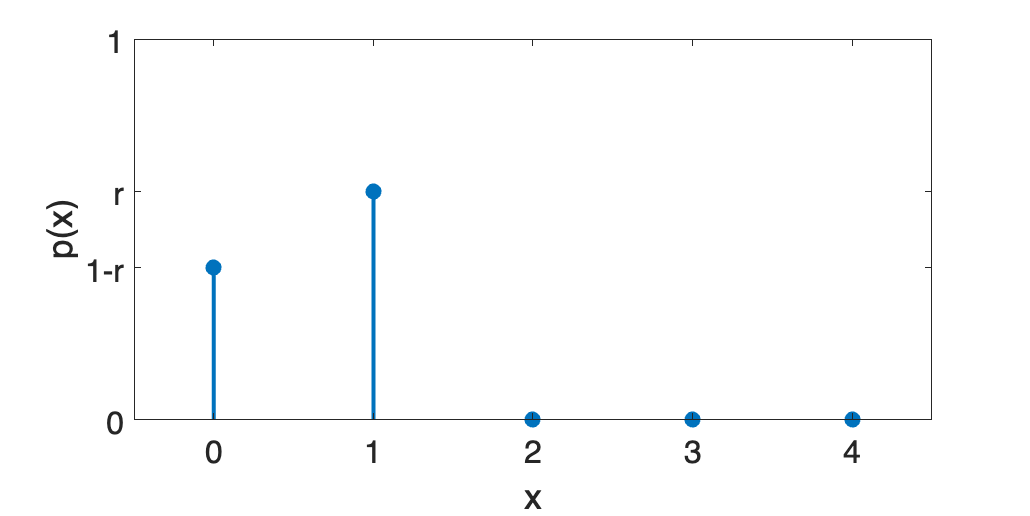
\includegraphics[width=.9\linewidth]{figures/bern.pmf.png}
  \caption{PMF.}
  \label{fig:bern:pmf}
\end{subfigure}\hfill
\begin{subfigure}{.5\textwidth}
  \centering
  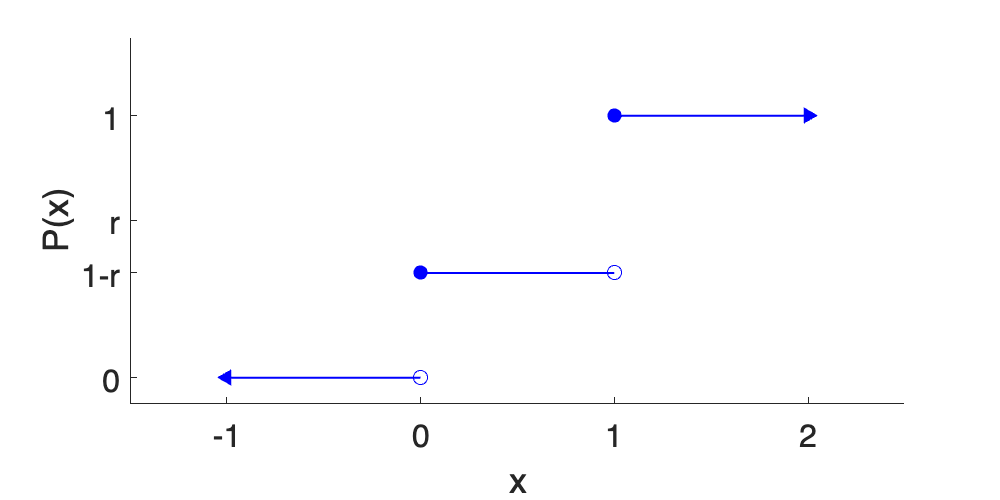
\includegraphics[width=.9\linewidth]{figures/bern.cdf.png}
  \caption{CDF.}
  \label{fig:bern:cdf}
\end{subfigure}
\caption[An example of the Bernoulli distribution.]{Bernoulli distribution.}
\label{fig:bern}
\end{figure}

The pmf and the cdf of the Bernoulli distribution can be seen on Figure \ref{fig:bern}.
We denote this distribution as $p(x) = \operatorname{Bernoulli}(x;r)$.
The expected value and the covariance of a Bernoulli random variable $X$ are

$$
E[X] = r, \qquad \operatorname{Var}[X] = r(1-r).
$$

In object tracking, we use Bernoulli random variables to model the existence of
an object at some time step $k$, which we will discuss in detail in the following
sections.
